\documentclass[]{Article}

\usepackage{amsmath}
\usepackage{amsfonts}
\usepackage{amssymb}

\usepackage{siunitx}
\usepackage{graphicx}

\author{Sawaiz Syed}
\title{SiPM MPPC Sensor Circuit}

\begin{document}
	
\maketitle
	
The main objective of this board was to take the example schematic from Hamamatsu that they use in their example board, and create a modular, lower cost, and easily expandable array of sensors. Another intention is to test how many sensors can be run from one power supply module as that component is that majority of the cost.

\begin{figure}[h!]
	\centering
	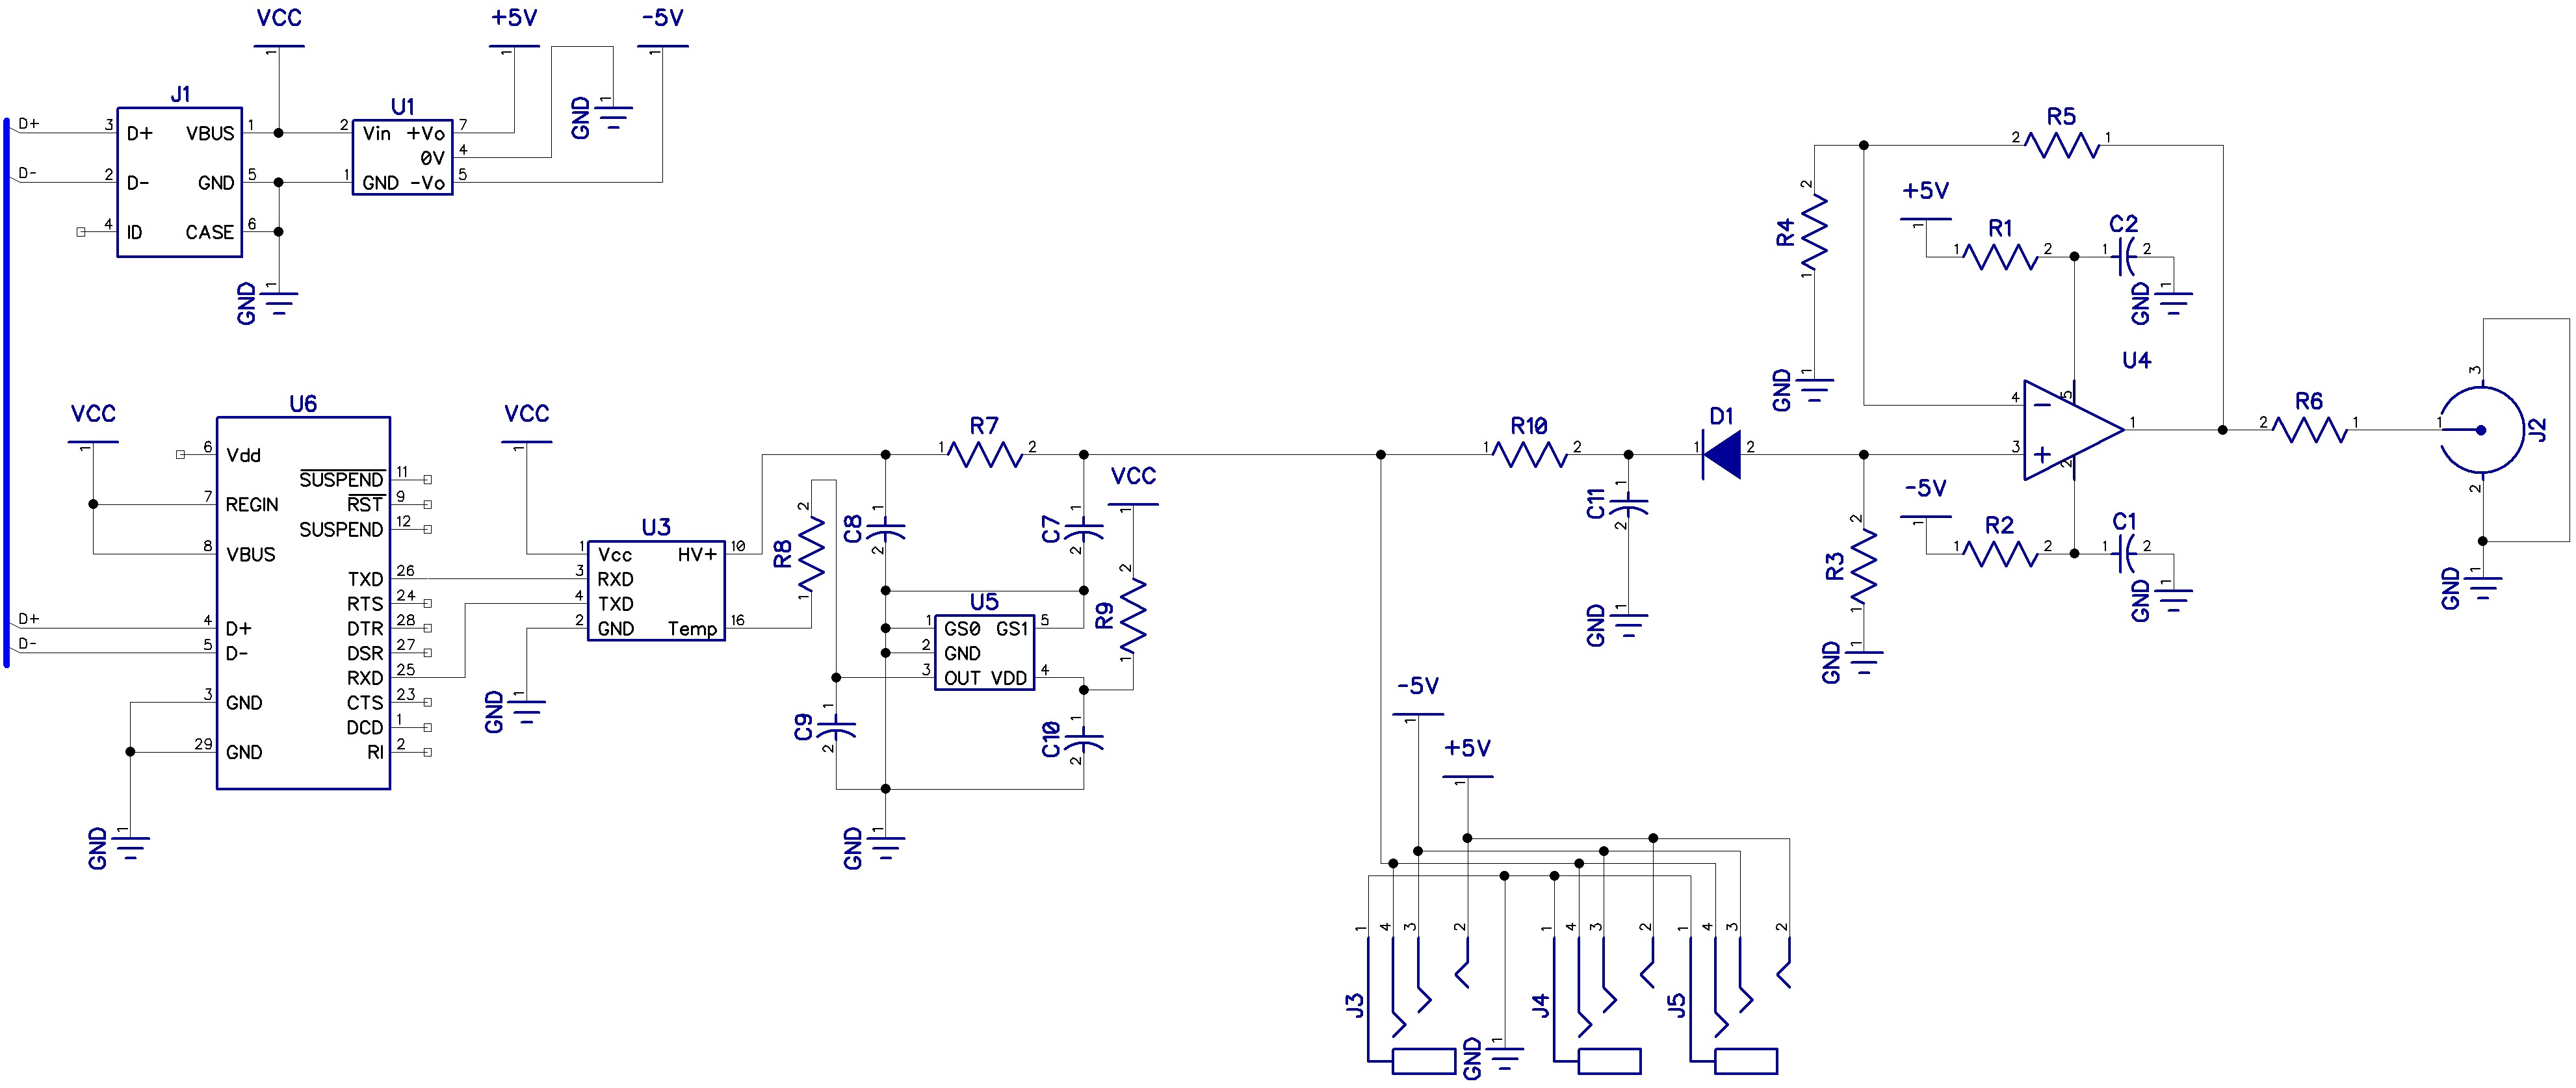
\includegraphics[width=\textwidth]{assets/sipm}
	\caption{The entire circuit diagram.}
\end{figure}

The circuit begins with a USB port, this provides the interface with the USB to UART chip that communicates with the HV power supply, allowing the user to set the voltage, and monitor the temperature sensor. The USB port also provides power to all the subsystems of the assembly, removing the need for any external power supply save the computer (or inexpensive cell phone charger adapter).

The power is initially routed to the $\pm$\SI{5}{\volt} converter. This integrated, switch mode power supply takes the +\SI{5}{\volt} USB power input and outputs $\pm$\SI{5}{\volt} with approximately \SI{40}{\milli\volt} of ripple. This power supply is only used for powering the Op-Amps as there is a \SI{200}{\milli\ampere} max current rating. The direct USB port \SI{5}{\volt} is used for all other parts.

\begin{figure}[h!]
	\centering
	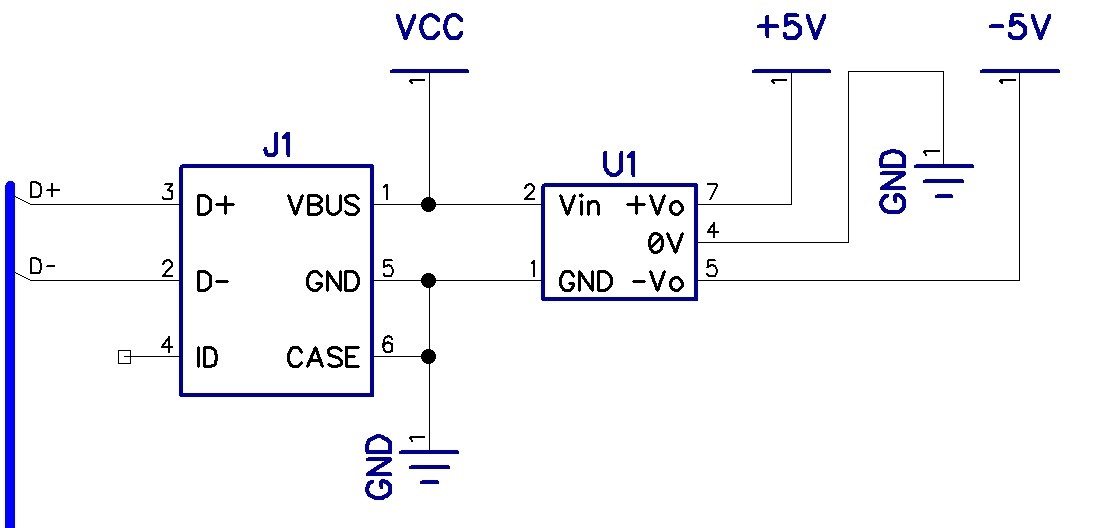
\includegraphics[width=\textwidth]{assets/power}
	\caption{USB port and $\pm$\SI{5}{\volt} converter.}
\end{figure}


The data lines from the USB port run to the CP2102 chip, capable of giving a UART interface with no other circuitry needed. This connects to the Hamamatsu C11204-01 high voltage module. Which is coupled with a LM94201 analog temperature sensor that allows the module to vary the bias voltage depending on the ambient temperature. The surrounding capacitor and resistor sets clean and stabilize the HV output before it is sent out on cables.

\begin{figure}[h!]
	\centering
	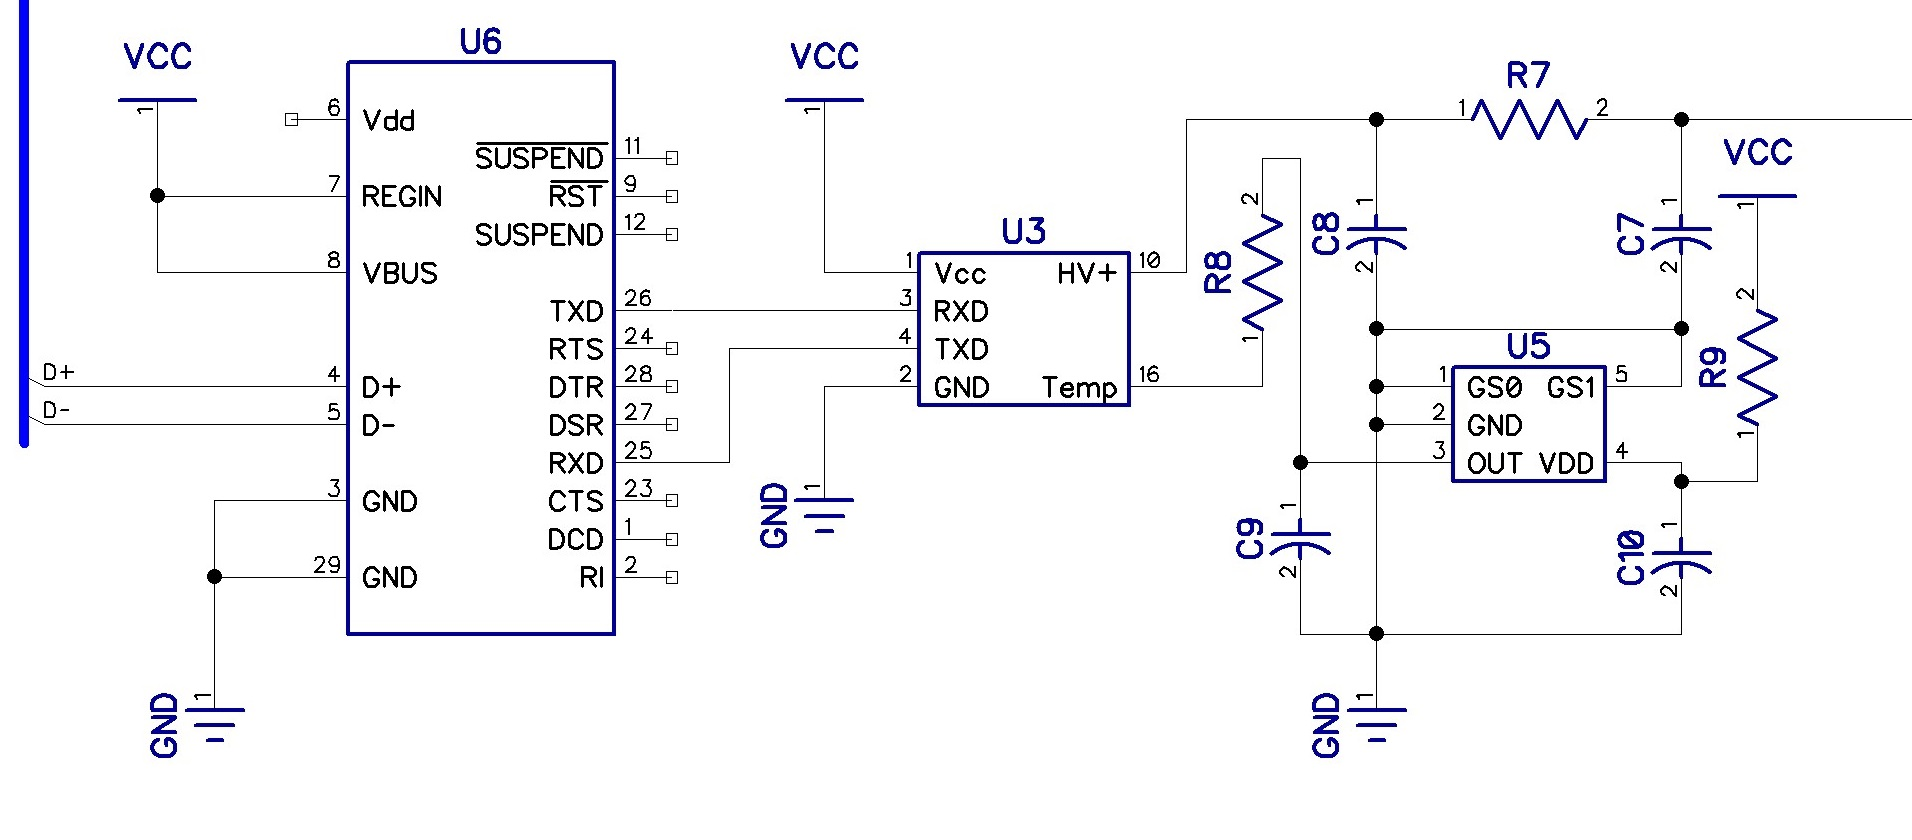
\includegraphics[width=\textwidth]{assets/uarthv}
	\caption{UART and High Voltage Supply.}
\end{figure}

Each sensor board, along with its connectors, has the MPPC, and a preamplifier. This allows the board to be very compact, measuring in at around \SI{50x12}{\milli\metre}. The sensor mounts to one side, and all the electronics attach to the other, leaving plenty of space for the sealing compounds to the empty sensor facing side.

\begin{figure}[h!]
	\centering
	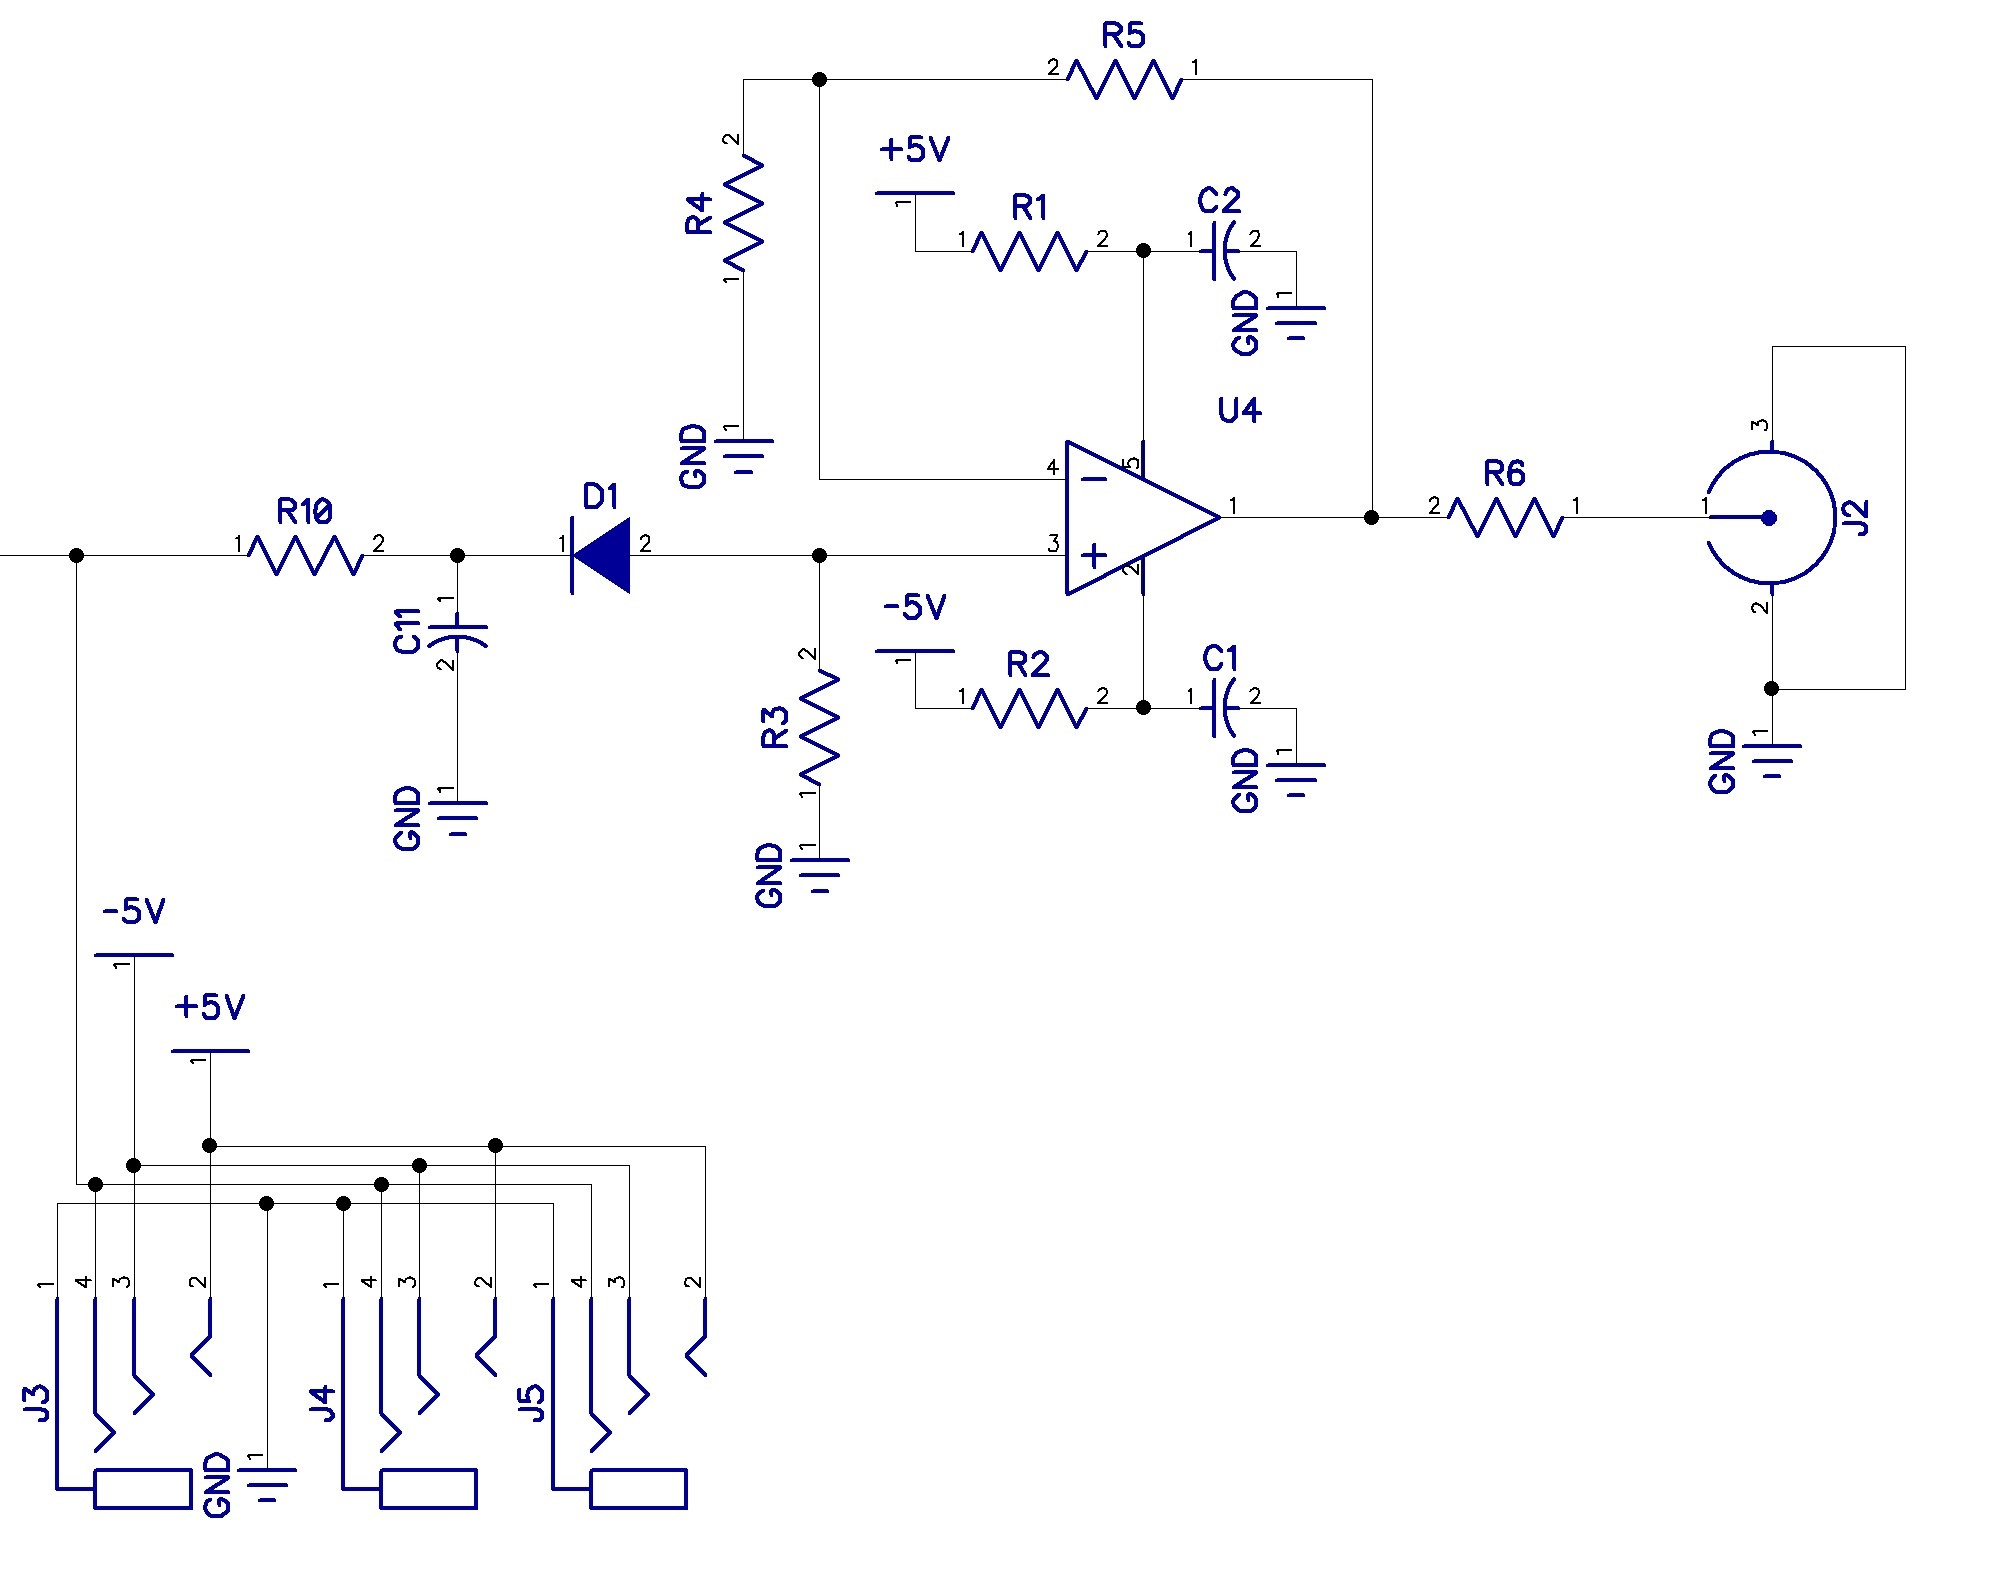
\includegraphics[width=\textwidth]{assets/amp}
	\caption{Op-Amp and connectors.}
\end{figure}

The cable selection was based primarily on cost and sourceability. The power cables were selected as TRRS jacks common on modern equipment for use as audio and microphone connectors. This allows us to use common cables, that are available in various lengths and are prefabricated. There is also two connectors on each sensor board, this allows the testing of daisy-chained sensors. This would first allow the use of less HV power supply modules, and also clean up wiring on the detector. The signal is fed through the common Hirsoe U.FL connector commonly found on laptop wireless cards. These cables are shielded, and capable of \SI{14}{\giga\hertz} signal transmission. The also happen to be the smallest, and most inexpensive of the commonly available coaxial cables.
	
\end{document}